\documentclass[phd]{byuprop}
% Options for this class include the following (* indicates default):
%
%   10pt -- 10 point font size
%   11pt -- 11 point font size
%   12pt (*) -- 12 point font size
%
%   ms -- produce a thesis proposal (off)
%   areaexam -- produce a research area overview (off)
%   phd -- produce a dissertation proposal (off)
%
%   singlespacing -- single-spaced lines
%   doublespacing -- double-spaced lines
%
%   layout -- show layout lines on the pages, helps with overfull boxes (off)
%   grid -- show a half-inch grid on every page, helps with printing (off)


% This command fixes my particular printer, which starts 0.03 inches too low,
% shifting the whole page down by that amount.  This shifts the document
% content up so that it comes out right when printed.
%
% Discovering this sort of behavior is best done by specifying the ``grid''
% option in the class parameters above.  It prints a 1/2 inch grid on every
% page.  You can then use a ruler to determine exactly what the printer is
% doing.
%
% Uncomment to shift content up (accounting for printer problems)
%\setlength{\voffset}{-.03in}

% Here we set things up for invisible hyperlinks in the document.  This makes
% the electronic version clickable without changing the way that the document
% prints.  It's useful, but optional.  Note that if you use latex instead of
% pdflatex, you should change "pdftex" to "ps2pdf".
\usepackage[
    pdftex,
    bookmarks=true,
    breaklinks=true,
    raiselinks=true,
    pdfborder={0 0 0},
    colorlinks=false,
    ]{hyperref}
    
\usepackage{caption}
\usepackage{subcaption}

% Rewrite the itemize, description, and enumerate environments to have more
% reasonable spacing:
\newcommand{\ItemSep}{\itemsep 0pt}
\let\oldenum=\enumerate
\renewcommand{\enumerate}{\oldenum \ItemSep}
\let\olditem=\itemize
\renewcommand{\itemize}{\olditem \ItemSep}
\let\olddesc=\description
\renewcommand{\description}{\olddesc \ItemSep}

% Get a little less fussy about word spacing on a line.  Sometimes produces
% ugly results, so keep your eyes peeled.
\sloppy

% Important settings for the byuprop class. %
%%%%%%%%%%%%%%%%%%%%%%%%%%%%%%%%%%%%%%%%%%%%%

% Because I use these things in more than one place, I created new commands for
% them.  I did not use \providecommand because I absolutely want LaTeX to error
% out if these already exist.
\newcommand{\Title}{
%Toward human-in-the-loop robotic path planning and navigation
Robot understanding of human intent : 
toward the collaboration in the human-robot team
}
\newcommand{\Author}{Daqing Yi}
\newcommand{\SubmissionMonth}{April}
\newcommand{\SubmissionYear}{2015}

% Take these from the commands defined above
\title{\Title}
\author{\Author}
\monthsubmitted{\SubmissionMonth}
\yearsubmitted{\SubmissionYear}

% Committee members
\committeechair{Michael~A.~Goodrich}
\committeemembera{Kevin~D.~Seppi}
\committeememberb{Randy~W.~Beard}
\committeememberc{Mark~J.~Clement}
\committeememberd{Parris~K.~Egbert}

% Department graduate coordinator
\graduatecoordinator{Quinn~Snell}

\documentabstract{%
% The proposal abstract should be 1 to 2 paragraphs.
%This document is an example of how to use the byuprop {\LaTeX} class file.  The class creates Ph.D. and Master's documents equally well, producing all appropriate preamble content and adhering precisely to the minimum formatting requirements.

%Note that there is a blank line between paragraphs, here.
Improvements in robot autonomy is changing the human-robot interaction from low-level manipulation to high-level task-based collaboration.
When the robot can independently and autonomously execute the tasks, the role of the human in a human-robot team is a collaborator and a task supervisor~\cite{Goodrich2013,Yi2014b}.
How the robot could understand the human's intent and how the robot responds to the environment dynamic and uncertainty determine the collaborative performance and the interaction experience.

In guiding the robot's decision making, the tasks are often modeled into optimization problems. 
As the made decision, an optimized solution leads how the robot should execute the task.


}

%%%%%%%%%%%%%%%%%%%%%%%%%%%%%%%%%%%%%%%%%%%%%

% Set up the internal PDF information so that it becomes part of the document
% metadata.  The pdfinfo command will display this. Be sure to set the document
% type and add your own keywords.
\hypersetup{%
    pdftitle=\Title,%
    pdfauthor=\Author,%
    %pdfsubject={Document Type, BYU CS Department: %
    %            Submitted \SubmissionMonth~\SubmissionYear, Created \today},%
    pdfsubject={PhD Proposal, BYU CS Department: %
                Submitted \SubmissionMonth~\SubmissionYear, Created \today},%
    pdfkeywords={Multi-objective optimization, Human-robot collaboration, Particle swarm optimization},%
}

% These packages allow the bibliography to be sorted alphabetically and allow references to more than one paper to be sorted and compressed (i.e. instead of [5,2,4,6] you get [2,4-6])
\usepackage[numbers,sort&compress]{natbib}
\usepackage{hyperref}

% Additional packages required for your specific thesis go here. I've left some I use as examples.
\usepackage{graphicx}
\usepackage{pdfsync}

\begin{document}

% Produce the preamble
\maketitle

%%%%%%%%%%%%%%%%%%%%%%%%%%%%%%%%%%%%%%%%%%%%%%%%%%%%%%%%%%%%%%%%%%%%%%%%%%%%%%%
\section{Introduction}
% 1-2 pages
% Answers:
% 1) What problem do you want to solve?
% 2) Who cares about this problem and why?

Although the robot intelligence is made by simulating human rationality, the ways how robot and the human think are still very different.
The human is expertized at making qualitative decision, from low-level movement to high-level reasoning.
While the robot shows great strength of solving quantitative problem, like high data-processing speed, high precisely repeated motion and etc.
In organizing the human and the robot in a team, the difference between the human and the robot should be considered in order to maximize the team performance.
When the human and the robot collaborate together, they are usually assigned different roles.
The human works on the high level, including high-level planning and scheduling, splitting the task into subtasks for different teammates, reacting to the situation changes.  
The robot works on the lower level, including low-level planning and task execution.

In a collaborative team, the shared mental model helps explaining the team functioning~\cite{Jonker:2010:SMM:2018118.2018128}.



\begin{figure}[hbtp]
\centering
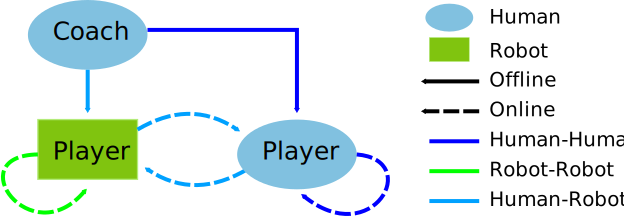
\includegraphics[width=0.7\linewidth]{./fig/team_info_flow.pdf}
\caption{The information flow in the team.}
\label{fig:team_info_flow}
\end{figure}


The mutual understanding in the collaboration between the human and the robot is important to the team performance.
[Discuss the influence of bad mutual understanding]
[priori + online]
There are a few methods to help the human understand the robot, like training and interactive display.
Having the robot understand the human is more difficult, because of the asymmetry in how the human and the robot process information.

%Like any collaboration in a shared environment, the mutual understanding and the information sharing between the robot and the human determine the team performance.
%By the training and a few interactive technologies, the human could better read what is happening to the robot.




%%%%%%%%%%%%%%%%%%%%%%%%%%%%%%%%%%%%%%%%%%%%%%%%%%%%%%%%%%%%%%%%%%%%%%%%%%%%%%%
\section{Related Work}

%%%%%%%%%%%%%%%%%%%%%%%%%%%%%%%%%%%%%%%%%%%%%%%%%%%%%%%%%%%%%%%%%%%%%%%%%%%%%%%
\subsection{Research Area Overview}
% Research Area Overview
% Describes the broad research area (citing the 20 most important papers)
% Should be about 3 pages and may be in the Introduction or Related Work
% sections or may be an appendix.


%%%%%%%%%%%%%%%%%%%%%%%%%%%%%%%%%%%%%%%%%%%%%%%%%%%%%%%%%%%%%%%%%%%%%%%%%%%%%%%
\subsection{Research-Related Work}
% Related Work
% 1-2 pages
% Answers:
% 3) What have others done to solve this problem and why is this inadequate?
%    (only a small overlap with the area exam from the introduction)




%%%%%%%%%%%%%%%%%%%%%%%%%%%%%%%%%%%%%%%%%%%%%%%%%%%%%%%%%%%%%%%%%%%%%%%%%%%%%%%
\section{Thesis Statement}
% 1 to 2 sentences

%%%%%%%%%%%%%%%%%%%%%%%%%%%%%%%%%%%%%%%%%%%%%%%%%%%%%%%%%%%%%%%%%%%%%%%%%%%%%%%
\section{Project Description}
% about 6-8 pages
% Answers:
% 4) What is your proposed solution to this problem?

\subsection{Modeling the human's intent}

\subsubsection{Reference path constrained optimal path planning}

\begin{figure}[hbtp]
\centering
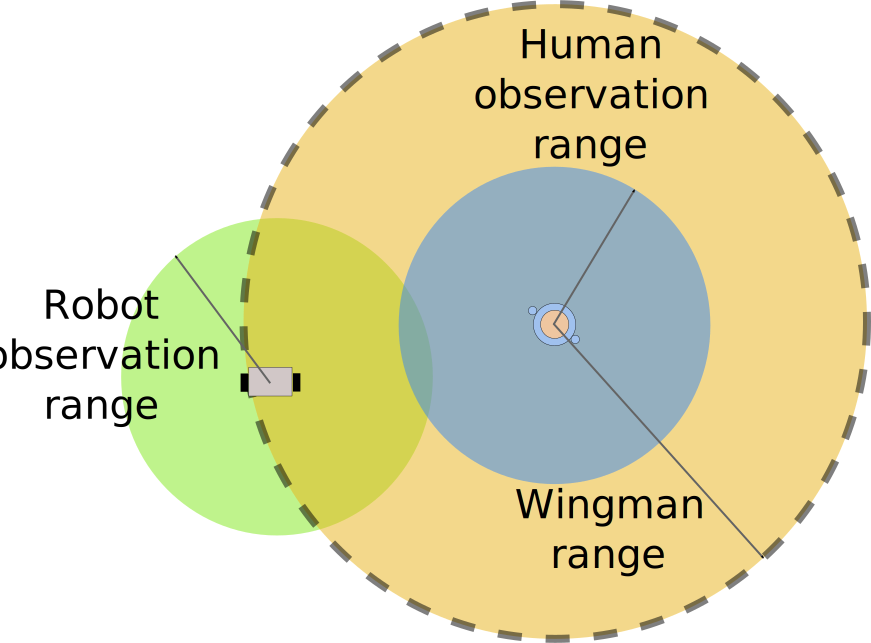
\includegraphics[width=0.5\linewidth]{./fig/Wingman.pdf}
\caption{A Robot Wingman Framework.}
\label{fig:Wingman}
\end{figure}

\begin{figure}[hbtp]
\centering
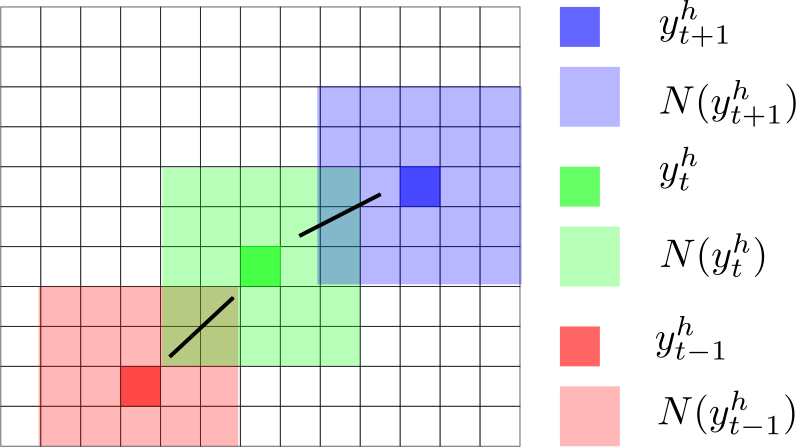
\includegraphics[width=0.6\linewidth]{./fig/humanConstraint}
\caption{How the multi-partite graph is obtained.}
\label{fig:humanConstraint}
\end{figure}

\begin{figure}[htbp]
\centering
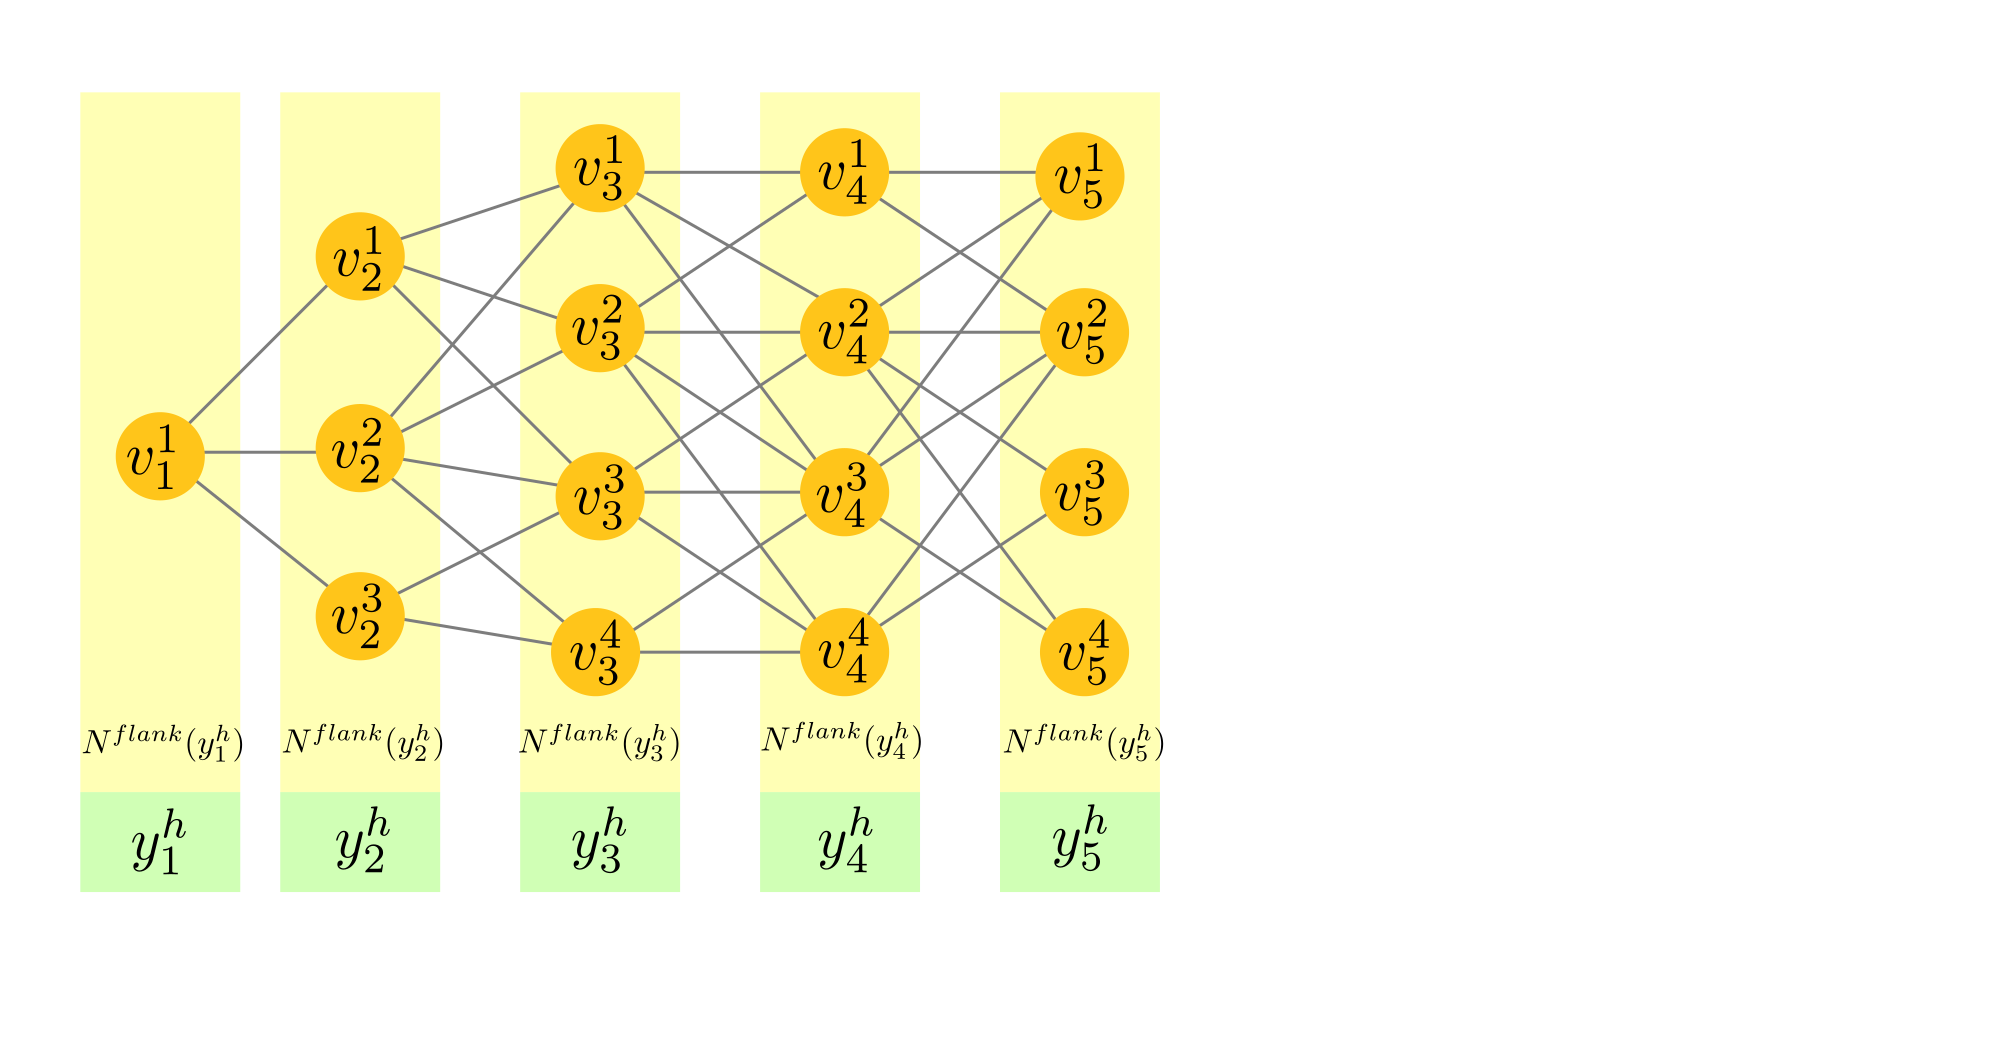
\includegraphics[width=0.6\linewidth]{./fig/MultiPartite.pdf}
\caption{A multi-partite graph from a human path constraint.}
\label{fig:MultiPartite}
\end{figure}

\subsubsection{Homotopy-based optimal path planning}

\begin{figure}[htbp]
	\centering
	\begin{subfigure}[t]{0.35\linewidth}
		\centering
		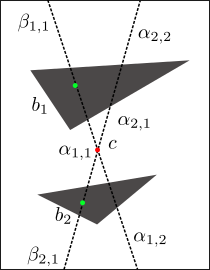
\includegraphics[width=\textwidth]{fig/obs_map.pdf}
		\caption{Decomposition of the map with obstacles.}
		\label{fig:obs_map:map}
	\end{subfigure}  
	%\\
	\begin{subfigure}[t]{0.35\linewidth}
		\centering
		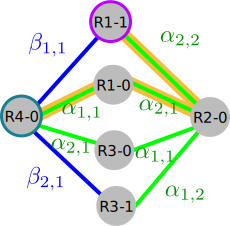
\includegraphics[width=\textwidth]{fig/obs_topology.pdf}
		\caption{The generated topological graph.}
		\label{fig:obs_map:topology}
	\end{subfigure}   
	\caption{Map with obstacles.}
	\label{fig:obs_map}
\end{figure}

\subsection{Multi-objective path planning}

\begin{figure}
\centering
\includegraphics[width=0.5\linewidth]{fig/Tchebycheff}
\caption{Tchebycheff method of finding Pareto front.}
\label{fig:Tchebycheff}
\end{figure}

\begin{figure}
	\centering
	\includegraphics[width=0.8\linewidth]{./fig/MORRTstar}
	\caption{Rapidly exploring process}
	\label{fig:MORRTstar}
\end{figure}

\subsection{Reaching a consensus}

\subsubsection{The consensus in a swarm}

\begin{figure}
\centering
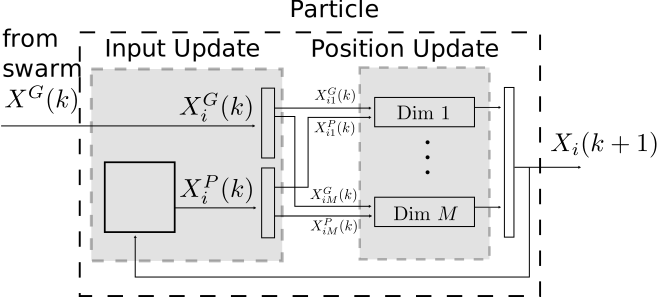
\includegraphics[width=0.7\linewidth]{./fig/particle_sys_flow.pdf}
\caption{System structure of Particle.}
\label{fig:sys:particle}
\end{figure}

\begin{figure}
\centering

\includegraphics[width=0.5\linewidth]{./fig/pso_sys_flow.pdf}
\caption{System structure of Swarm}
\label{fig:sys:swarm}
\end{figure}

\begin{figure}
\centering
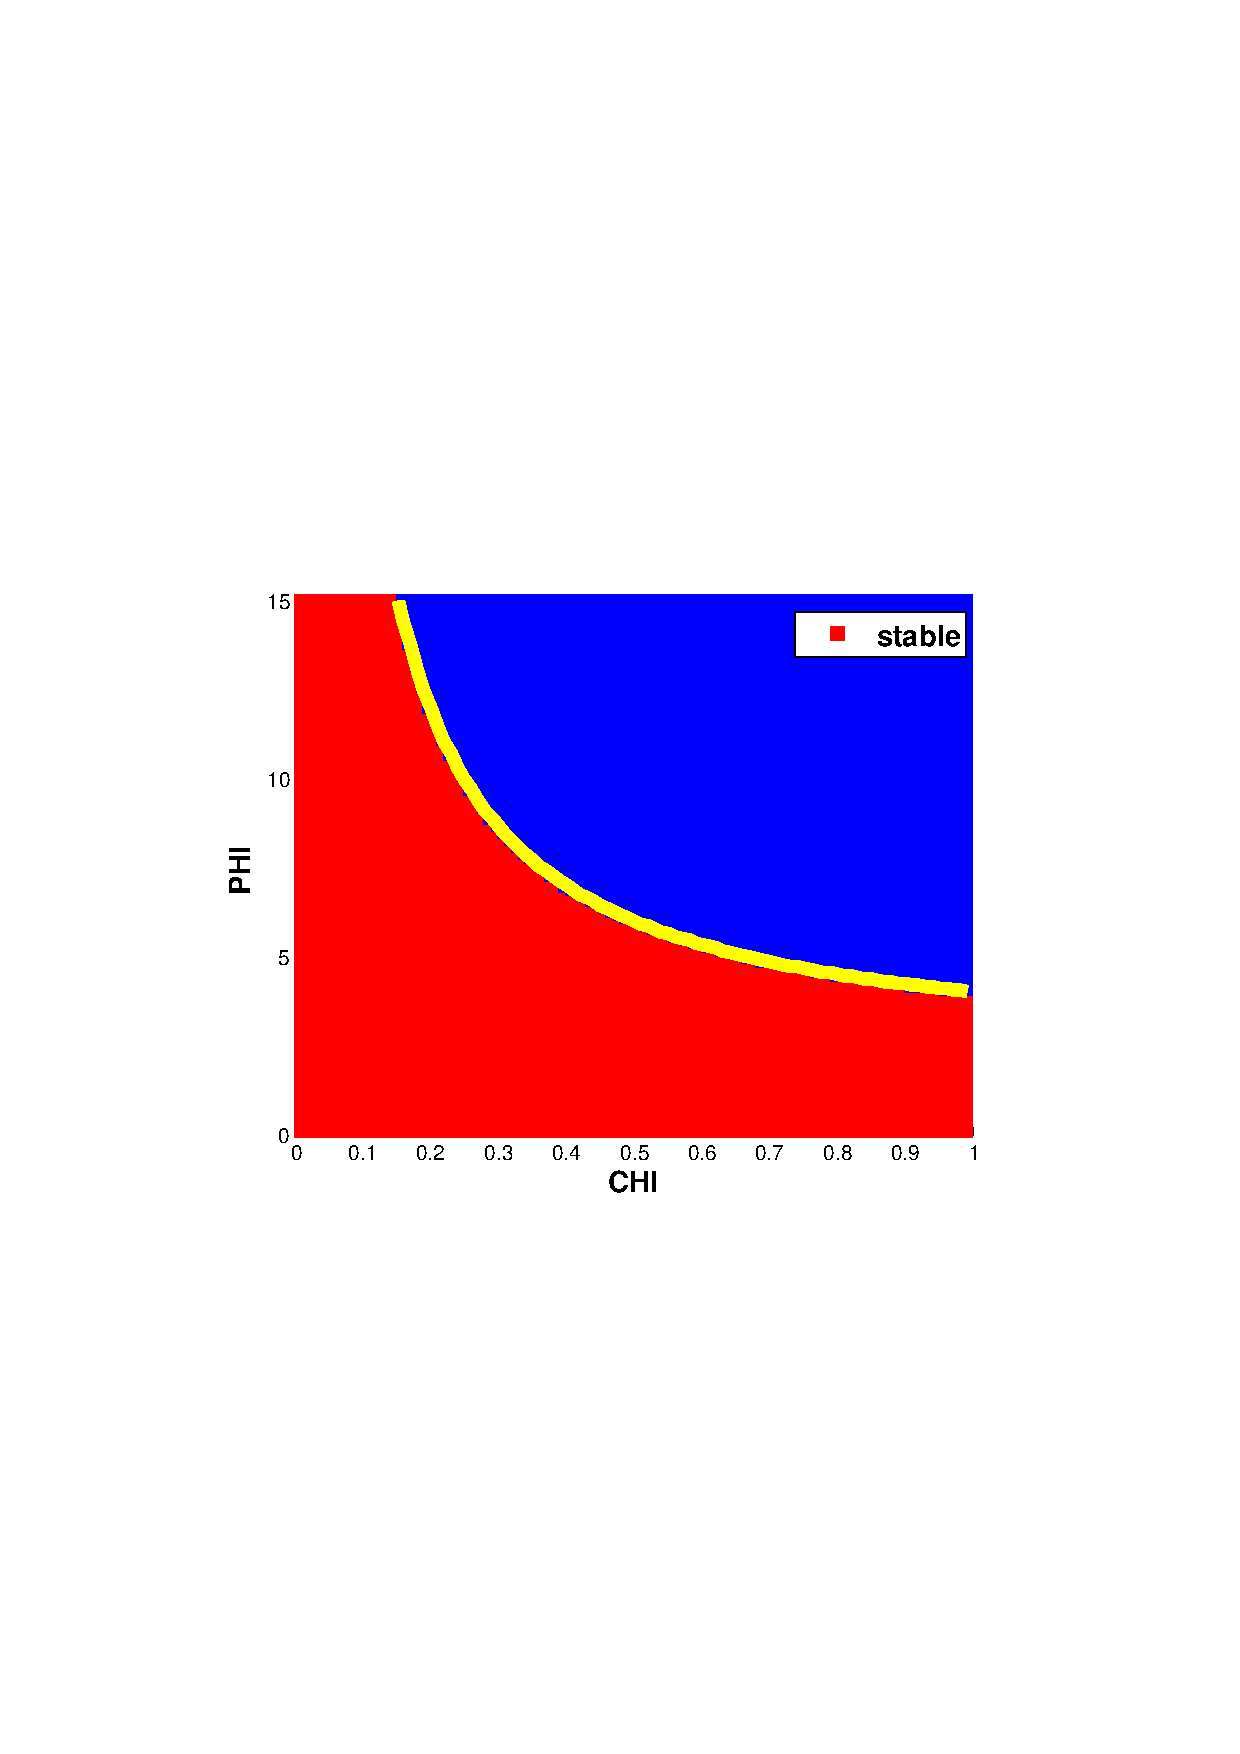
\includegraphics[width=0.5\linewidth]{./fig/param2.png}
\caption{Parameter space}
\label{fig:paramSpace}
\end{figure}

\begin{figure}
\centering
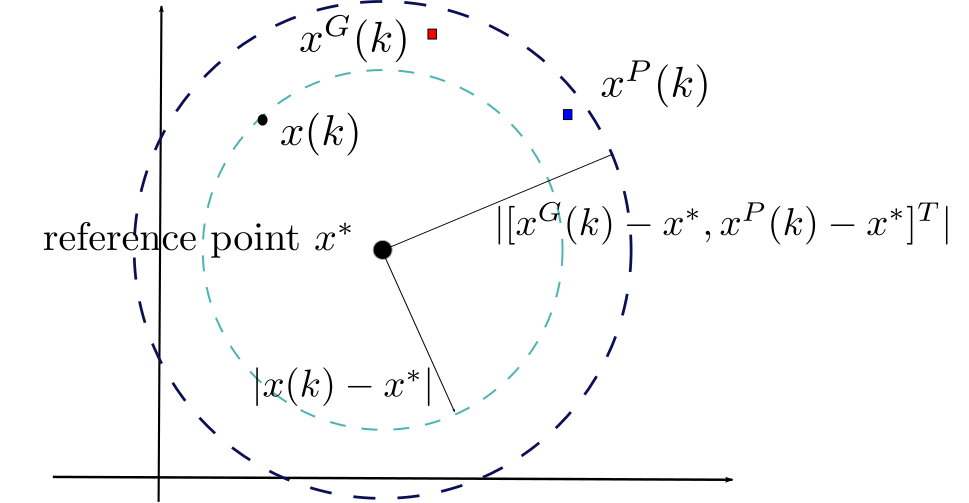
\includegraphics[width=0.6\linewidth]{./fig/boundary}
\caption{A bound on a particle's position by a reference point $ x^{*} $ from Equation %\eqref{eq:state_bound:conv}.
The ratio of two radii indicates $ \gamma $.}
\label{fig:boundary}
\end{figure}


\subsection{The consensus between human and robot}


\subsection{Including information uncertainty}



%%%%%%%%%%%%%%%%%%%%%%%%%%%%%%%%%%%%%%%%%%%%%%%%%%%%%%%%%%%%%%%%%%%%%%%%%%%%%%%
\section{Validation}
% 1-2 pages
% Answers:
% 5) How can you demonstrate that this is a good solution?

%%%%%%%%%%%%%%%%%%%%%%%%%%%%%%%%%%%%%%%%%%%%%%%%%%%%%%%%%%%%%%%%%%%%%%%%%%%%%%%
\section{Dissertation Schedule}
% about 1/2 page
% specifying dates for completion of major milestones, including potential
% papers and their submission dates

\begin{itemize}
\item Conference Paper: Toward Task-Based Mental Models of Human-Robot Teaming: A Bayesian Approach. (July 2013)
\item Conference Paper: Supporting task-oriented collaboration in human-robot teams using semantic-based path planning. (June 2014)
\item Conference Paper: Path Planning with a Human
Path Constraint. (October 2014)
\item Conference Paper: Input-to-state stable analysis on Particle Swarm Optimization. (July 2015)
\item Conference Paper: MORRF$^{*}$ : Sampling-Based Multi-Objective Motion Planning. (2015)
\item Conference Paper: Homotopy-Aware RRT$^{*}$ : Toward Human-Robot Topological Path-Planning. (2015)
\item Journal Paper: Understanding the Particle Swarm Optimization by component decomposition. (2015)
\item Submission of the dissertation to advisor ()
\item Submission of the dissertation to committee members ()
\item Dissertation Defense ()
\item Conference Paper:
\item Journal Paper: 
\end{itemize}

%%%%%%%%%%%%%%%%%%%%%%%%%%%%%%%%%%%%%%%%%%%%%%%%%%%%%%%%%%%%%%%%%%%%%%%%%%%%%%%
% Change these to reflect the bibliography style and bibtex database file you want to use
\bibliographystyle{plain}
\bibliography{proposal_ref}

\end{document}
